\newpage
\subsection{Indflydelse af basrefleksens placering}
Hullerne på kabinettets side gør det muligt, at placere de forskellige basreflekser forskellige steder i højtaleren. Teoretisk er der ikke blevet gennemgået nogle modeller der beskriver betydningen af basrefleksens placering; betydningen vil i stedet blive undersøgt empirisk.

For at holde variablerne under kontrol, så undersøges betydningen af placeringen først ved, at placere den lange basrefleks forskellige steder. Der blev herefter målt inde i selve basrefleksporten. Resultatet af dette ses nedenfor:
\begin{figure}[H]
	\centering
	\vspace{-12pt}
%	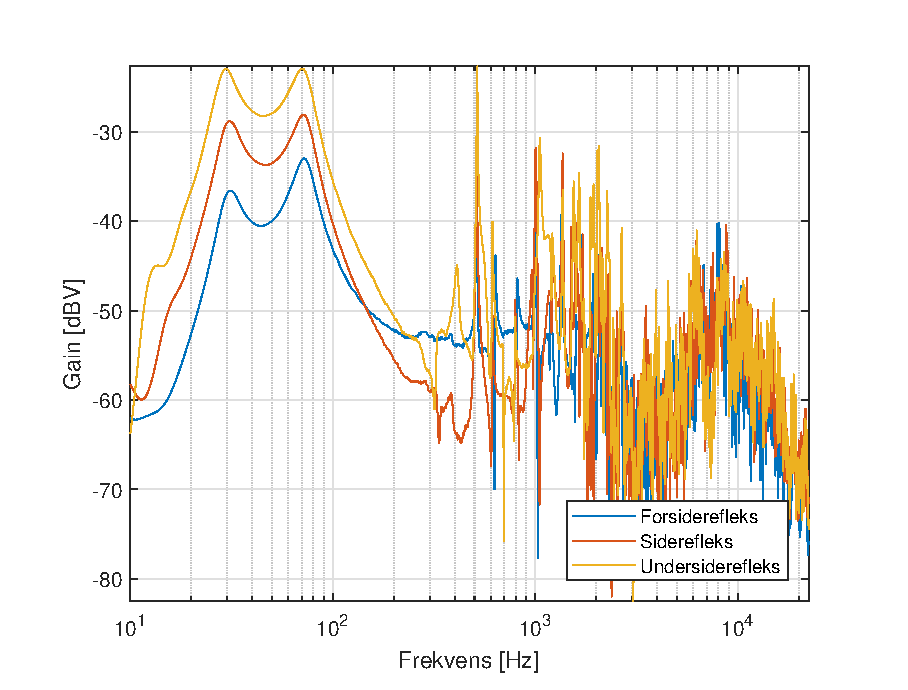
\includegraphics[width=\textwidth]{Pics/BassReflexPlacementLongReflex}
	\caption{Basrefleksens frekvenskarakteristik}
\end{figure}

Selvom frekvenskarakteristikken bliver svær at aflæse ved frekvenser over \SI{300}{\hertz} så forekommer der tre tydelige karakteristikker mellem \SI{20}{\hertz} til \SI{200}{\hertz}. Dette er basrefleksportens velkendte frekvenskarakteristikker - dog med forskellige amplituder.